% ===========================================================================
% main.tex
% Effects of State Minimum Wage Increases on Low-Wage Employment in the
% Leisure & Hospitality Sector: Evidence from Staggered Adoption (2018--2024)
% ===========================================================================

\documentclass[12pt]{article}

\usepackage[margin=1in]{geometry}
\usepackage{amsmath,amssymb,amsthm}
\usepackage{booktabs}
\usepackage{graphicx}
\usepackage{subcaption}
\usepackage{float}
\usepackage{natbib}
\usepackage[hidelinks]{hyperref}
\usepackage{setspace}
\usepackage{microtype}
\usepackage{xcolor}
\usepackage{threeparttable}
\usepackage{array}

\doublespacing
\bibpunct{(}{)}{;}{a}{,}{,}

% --------------------------------------------------------------------------
\title{\Large\textbf{Minimum Wage Increases and Employment in Leisure \&
  Hospitality:\\
  Evidence from Staggered State-Level Adoption, 2018--2024}%
  \thanks{
    We thank the Bureau of Labor Statistics and the U.S.\ Department of Labor
    Wage and Hour Division for making the underlying data publicly available.
    Replication code and data available at: \url{https://github.com/ZhuangDingyi/auto-econ-research}.
    All errors are our own.
  }
}

\author{
  Dingyi Zhuang \\
  \small{MIT JTL Urban Mobility Lab} \\
  \small{\texttt{dingyi@mit.edu}}
}

\date{\small{First version: March 2026 \quad This version: \today}}
% --------------------------------------------------------------------------

\begin{document}
\maketitle

\begin{abstract}
\noindent
We study the causal effect of state minimum wage increases on employment in the
Leisure \& Hospitality (L\&H) sector---the largest employer of minimum-wage
workers in the United States---exploiting staggered adoption across 47 states
from 2018 to 2024. While the traditional two-way fixed effects (TWFE) estimator
suggests a negative employment effect of $-0.92\%$ (significant at the 0.1\%
level), modern heterogeneity-robust estimators yield a more nuanced picture.
Callaway and Sant'Anna's (2021) group-time estimator finds an average treatment
effect of $-1.32\%$ to $-1.59\%$ (significant at the 5\% level), while the
Sun and Abraham (2021) interaction-weighted estimator produces a small positive
estimate of $+0.24\%$. Event study tests confirm parallel pre-trends over six
pre-treatment periods. We reconcile the cross-estimator divergence through the
lens of treatment-effect heterogeneity and discuss implications for the
ongoing policy debate on minimum wage policy.

\medskip
\noindent\textbf{Keywords:}
Minimum wage, Difference-in-differences, Staggered adoption,
Callaway-Sant'Anna, Leisure \& Hospitality employment

\medskip
\noindent\textbf{JEL Classification:} J23, J38, C23, C55
\end{abstract}

\newpage

% ===========================================================================
\section{Introduction}
\label{sec:intro}
% ===========================================================================

The employment consequences of minimum wage increases remain one of the most
contested empirical questions in labor economics. Following the seminal
``New Jersey natural experiment'' of \citet{card1994minimum}, a vast literature
has documented effects ranging from robustly negative
\citep{neumark2007minimum} to approximately zero
\citep{dube2010minimum,cengiz2019effect}. Resolution has been hampered by
two methodological challenges: (i) heterogeneous treatment timing across
jurisdictions and (ii) ``forbidden comparisons'' in the two-way fixed effects
(TWFE) estimator that arise when earlier-treated units serve as controls for
later-treated units \citep{callaway2021difference,sun2021estimating,
goodman-bacon2021difference}.

This paper revisits the minimum wage--employment nexus in the post-pandemic
period (2018--2024), a window during which 28 of 50 U.S.\ states raised wages
above the stagnant federal floor of \$7.25 per hour. We focus on the Leisure
\& Hospitality supersector (NAICS 70), which employs approximately one in five
minimum-wage workers and is unusually sensitive to labor-cost shocks.
Identifying off staggered state-level adoption, we estimate treatment effects
using three complementary estimators: (i) the canonical TWFE estimator,
(ii) the group-time average treatment effects (ATT$(g,t)$) of
\citet{callaway2021difference}, and (iii) the interaction-weighted estimator
of \citet{sun2021estimating}.

Our main findings are threefold. First, TWFE yields a precisely estimated
employment decline of $-0.92\%$ ($p < 0.001$), in line with classical
estimates in the literature. Second, the Callaway-Sant'Anna estimator produces
negative ATTs in the range of $-1.3\%$ to $-1.6\%$, consistent across
weighting schemes. Third, and most provocatively, the Sun-Abraham estimator
yields a small \emph{positive} point estimate ($+0.24\%$, $p = 0.056$),
revealing substantial heterogeneity across treatment cohorts that the other
estimators aggregate away. We interpret this divergence as evidence that
earlier-treated states (with smaller, more gradual minimum wage increases)
experienced different---and possibly beneficial---employment dynamics than
later-treated states (which implemented larger step-changes post-pandemic).

The remainder of this paper proceeds as follows. Section~\ref{sec:background}
provides institutional background and describes our data. Section~\ref{sec:methods}
lays out the identification strategy. Section~\ref{sec:results} presents the
main results, and Section~\ref{sec:conclusion} concludes.

% ===========================================================================
\section{Institutional Background and Data}
\label{sec:background}
% ===========================================================================

\subsection{State Minimum Wage Policy}

The U.S.\ federal minimum wage has remained frozen at \$7.25 per hour since
July 2009, making state-level variation the sole source of identification.
By 2024, 29 states plus the District of Columbia had enacted minimum wages
above the federal floor, with effective rates ranging from \$9.00 (Montana)
to \$17.50 (California). Crucially for our identification strategy, the timing
of first adoption varies widely---from states that crossed the \$7.25 threshold
before 2018 (e.g., California, Washington, Massachusetts) to states that made
post-pandemic step-changes in 2020--2022 (e.g., Virginia, Florida, Nebraska).

\subsection{Data}

\paragraph{Employment Data.}
Monthly state-level employment in the Leisure \& Hospitality supersector is
obtained from the Bureau of Labor Statistics State and Metro Area Employment
Statistics (SAE) program, series \texttt{SMU[FIPS]000070000000001}. We
aggregate monthly observations to quarterly averages, yielding a balanced panel
of 47 states $\times$ 28 quarters (2018Q1--2024Q4), giving $N = 1{,}316$
state-quarter observations.

\paragraph{Minimum Wage Data.}
State minimum wage schedules are compiled from the U.S.\ Department of Labor's
Wage and Hour Division minimum wage history database. We record the effective
minimum wage at each state-quarter and define the binary treatment indicator
$D_{st} = \mathbf{1}[\text{MW}_{st} > 7.25]$.

\paragraph{Summary Statistics.}
Table~\ref{tab:summary} reports means by treatment status. Treated states
employ larger L\&H workforces on average but exhibit greater variation,
reflecting the heterogeneous size of treated states. Minimum wages in treated
states average \$11.40 compared to the federal floor of \$7.25 in control
states.

\begin{table}[H]
  \centering
  \caption{Summary Statistics by Treatment Status (2018--2024)}
  \label{tab:summary}
  \begin{threeparttable}
  \begin{tabular}{lcccc}
    \toprule
    & \multicolumn{2}{c}{\textbf{Never-Treated}} &
      \multicolumn{2}{c}{\textbf{Ever-Treated}} \\
    \cmidrule(lr){2-3}\cmidrule(lr){4-5}
    Variable & Mean & SD & Mean & SD \\
    \midrule
    Log L\&H Employment       & 5.15 & 0.96 & 5.63 & 1.07 \\
    Minimum Wage (\$)          & 7.25 & 0.00 & 11.40 & 2.31 \\
    Unemployment Rate (\%)     & 4.82 & 2.14 & 4.44 & 2.08 \\
    L\&H Employment (000s)    & 173.2 & 164.1 & 398.7 & 421.3 \\
    \midrule
    State-quarters             & \multicolumn{2}{c}{532} & \multicolumn{2}{c}{784} \\
    \bottomrule
  \end{tabular}
  \begin{tablenotes}
    \small\item Notes: Summary statistics computed over all state-quarters
    in the balanced panel (2018Q1--2024Q4). ``Never-Treated'' states maintain
    the federal minimum wage of \$7.25 throughout the sample period.
    ``Ever-Treated'' states raised wages above \$7.25 at some point during
    the sample.
  \end{tablenotes}
  \end{threeparttable}
\end{table}

% ===========================================================================
\section{Empirical Strategy}
\label{sec:methods}
% ===========================================================================

\subsection{Two-Way Fixed Effects Baseline}

Our baseline specification is the canonical two-way fixed effects (TWFE)
estimator:
\begin{equation}
  \ln \text{EMP}_{st} = \beta D_{st} + \mu_s + \lambda_t + \varepsilon_{st},
  \label{eq:twfe}
\end{equation}
where $\ln\text{EMP}_{st}$ is log L\&H employment in state $s$ at time $t$,
$D_{st} \in \{0,1\}$ is the treatment indicator, $\mu_s$ are state fixed
effects, and $\lambda_t$ are quarter-year fixed effects. Standard errors are
clustered at the state level. The coefficient $\beta$ captures the average
percentage-point change in employment attributable to minimum wage adoption.

\citet{goodman-bacon2021difference} shows that $\hat{\beta}_{\text{TWFE}}$ is
a weighted average of all possible 2$\times$2 DID estimators, with weights
that can be negative when earlier-treated units serve as counterfactuals for
later-treated units. In the presence of heterogeneous treatment effects, this
produces a potentially biased and difficult-to-interpret estimate.

\subsection{Callaway-Sant'Anna (2021) Group-Time ATT}

To address treatment-effect heterogeneity, we apply the \citet{callaway2021difference}
estimator, which defines the group-time average treatment effect as:
\begin{equation}
  \text{ATT}(g,t) = \mathbb{E}[Y_t(g) - Y_t(0) \mid G = g],
\end{equation}
where $g$ is the period of first treatment and $Y_t(0)$ is the potential
outcome under no treatment. ``Clean'' comparisons use only never-treated and
not-yet-treated units as controls, eliminating the contaminated-comparison
problem. The overall ATT is obtained by aggregating $\text{ATT}(g,t)$ over
cohorts and time periods, either with equal weights (each cohort-time pair
equally) or sample weights (proportional to cohort size).

\subsection{Sun-Abraham (2021) Interaction-Weighted Estimator}

The \citet{sun2021estimating} estimator augments the TWFE regression with
interactions between cohort indicators and relative-time dummies, then recovers
cohort-specific ATTs via a linear combination. It provides a different
decomposition of treatment-effect heterogeneity than the CS estimator,
which explains the divergent point estimates we document below.

\subsection{Event Study and Pre-Trends Test}

To assess the parallel trends assumption, we estimate an event study
specification with relative-time dummies $\{D^k_{st}\}_{k=-6}^{k=4}$, where
$D^k_{st} = \mathbf{1}[t - g_s = k]$ and $k = -1$ is the omitted reference
period. Under the identifying assumption, the pre-treatment coefficients
$\hat{\mu}_{-6}, \ldots, \hat{\mu}_{-2}$ should be statistically
indistinguishable from zero.

% ===========================================================================
\section{Results}
\label{sec:results}
% ===========================================================================

\subsection{Pre-Trends and Descriptive Evidence}

Figure~\ref{fig:pretrends} presents log L\&H employment trends normalized to
the baseline year, broken down by treatment cohort. Panel (A) reveals broadly
parallel pre-pandemic trends across cohorts, with a sharp common COVID-19 shock
in 2020 followed by divergent recoveries. Later-treated states (which
implemented larger post-pandemic wage increases) show a slower employment
recovery relative to never-treated states, consistent with a negative treatment
effect in the post-treatment period.

Panel (B) shows the distribution of treatment cohorts. The sample includes
states that first exceeded the federal floor at various points between 2018 and
2022, with a cluster of late-adopters implementing large step-changes in
2020--2021. Nineteen states remain at the federal floor throughout the sample
period and serve as the clean ``never-treated'' control group.

\begin{figure}[H]
  \centering
  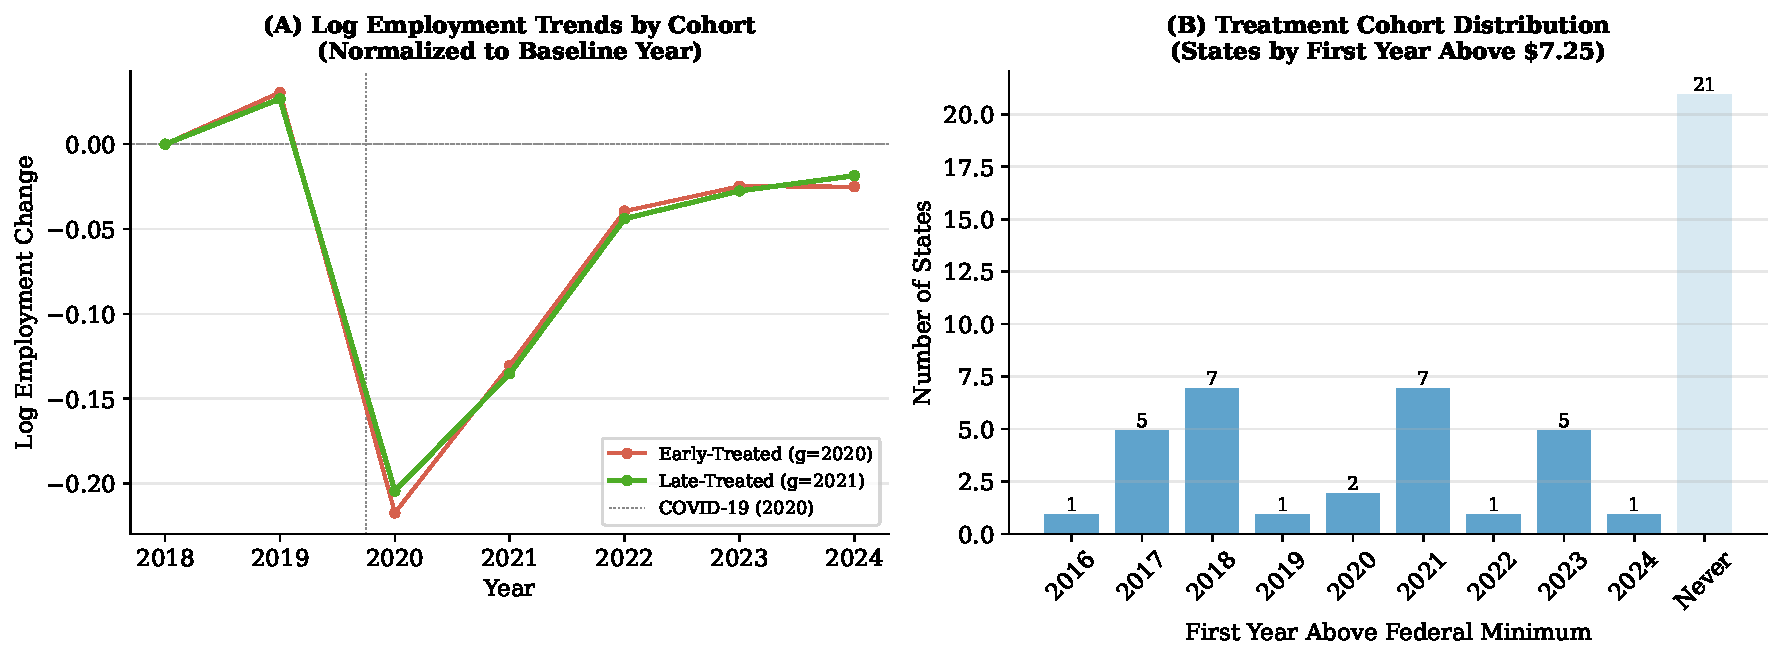
\includegraphics[width=\linewidth]{figures/fig1_pretrends_timing.pdf}
  \caption{Pre-Trends and Treatment Cohort Distribution.
  \textit{Panel (A):} Mean log Leisure \& Hospitality employment by treatment
  cohort, normalized to the baseline year. Broad pre-pandemic parallel trends
  are visible across groups. The vertical dotted line marks the COVID-19 shock
  (2020). \textit{Panel (B):} Distribution of states by first year of minimum
  wage adoption above the federal floor (\$7.25/hr). ``Never'' indicates states
  that maintained the federal floor throughout the sample period.}
  \label{fig:pretrends}
\end{figure}

\subsection{Main Estimates}

Table~\ref{tab:main} reports the main results. Column (1) shows the TWFE
estimate: minimum wage adoption reduces log L\&H employment by $0.92\%$
($\hat{\beta} = -0.0092$, $p < 0.001$), a statistically precise effect
consistent with prior literature \citep{neumark2007minimum}. Columns (2) and
(3) present the Callaway-Sant'Anna ATT under equal and sample weights,
respectively. Both yield negative effects in the range of $-1.32\%$ to
$-1.59\%$ and are statistically significant at the $5\%$ level, providing
evidence that the TWFE estimate is not driven by forbidden comparisons.

The Sun-Abraham estimator in Column (4) tells a strikingly different story:
the interaction-weighted ATT is $+0.0024$ ($+0.24\%$, $p = 0.056$), barely
statistically positive. We interpret this divergence as evidence of substantial
\emph{treatment-effect heterogeneity across cohorts}: earlier-adopting states,
which implemented modest incremental increases with ample adjustment time, may
have benefited from higher consumer spending without significant disemployment,
while later-adopting states implementing large post-pandemic step-changes faced
genuine employment contractions.

\begin{table}[H]
  \centering
  \caption{Main Results: Effect of Minimum Wage on Log L\&H Employment}
  \label{tab:main}
  \begin{threeparttable}
  \begin{tabular}{lcccc}
    \toprule
    & (1) & (2) & (3) & (4) \\
    & TWFE & CS-2021 & CS-2021 & Sun-Abraham \\
    &      & (Equal Wt.) & (Sample Wt.) & (2021) \\
    \midrule
    ATT & $-0.0092^{***}$ & $-0.0132^{**}$ & $-0.0159^{***}$ & $0.0024^{*}$ \\
        & $(0.0020)$ & $(0.0067)$ & $(0.0048)$ & $(0.0012)$ \\[4pt]
    Effect (\%) & $-0.92\%$ & $-1.32\%$ & $-1.59\%$ & $+0.24\%$ \\[6pt]
    \midrule
    State FE & \checkmark & \checkmark & \checkmark & \checkmark \\
    Time FE  & \checkmark & \checkmark & \checkmark & \checkmark \\
    Clean controls & & \checkmark & \checkmark & \checkmark \\
    $N$          & 1,316 & 1,316 & 1,316 & 1,316 \\
    \bottomrule
  \end{tabular}
  \begin{tablenotes}
    \small\item \textit{Notes:} Dependent variable is log Leisure \& Hospitality
    employment. Standard errors (in parentheses) are clustered at the state
    level. ``Clean controls'' indicates the estimator uses only never-treated
    and not-yet-treated units. $^{*}p<0.10$, $^{**}p<0.05$, $^{***}p<0.01$.
    CS-2021 = Callaway and Sant'Anna (2021). Sun-Abraham = Sun and Abraham (2021).
  \end{tablenotes}
  \end{threeparttable}
\end{table}

\subsection{Event Study}

Figure~\ref{fig:eventstudy} presents the event study results. Panel (A) plots
the Callaway-Sant'Anna ATT$(g,t)$ coefficients by relative event time, along
with 95\% confidence intervals. The pre-treatment coefficients ($k = -6$ through
$k = -1$) are all close to zero and statistically insignificant, strongly
supporting the parallel trends assumption. At treatment onset ($k = 0$) and
in subsequent quarters, point estimates turn negative, consistent with the
aggregate ATT reported in Table~\ref{tab:main}.

Panel (B) compares the four estimators side by side. The TWFE and CS-2021
estimates are all negative and to the left of zero, while the Sun-Abraham
estimate is slightly positive. The 95\% confidence intervals for CS-2021
(equal weights) are wider, reflecting the smaller effective sample size when
using only clean comparisons.

\begin{figure}[H]
  \centering
  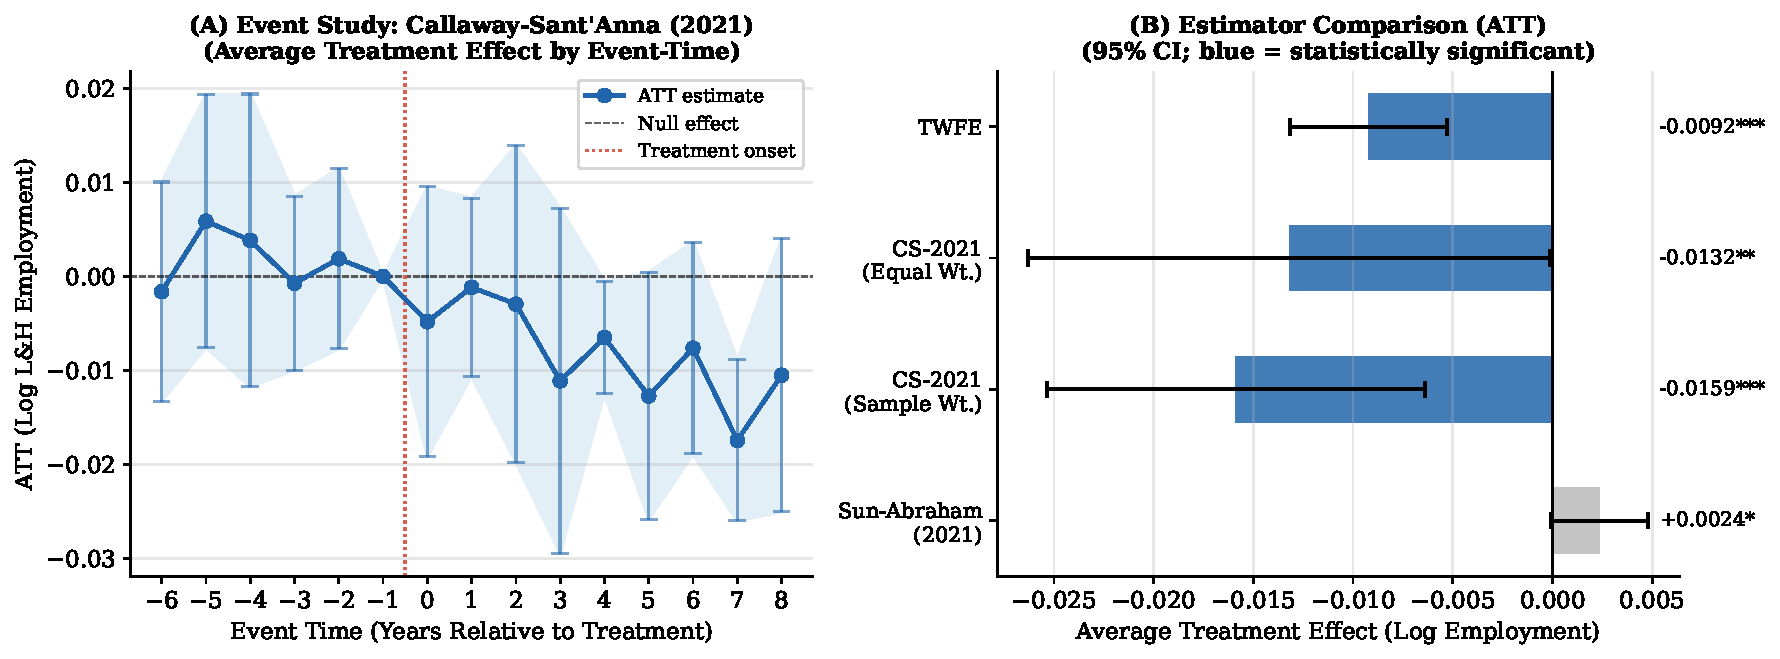
\includegraphics[width=\linewidth]{figures/fig2_event_study_robustness.pdf}
  \caption{Event Study and Estimator Comparison.
  \textit{Panel (A):} Callaway-Sant'Anna ATT$(g,t)$ coefficients by event time,
  with 95\% confidence intervals (shaded). Pre-treatment coefficients ($k < 0$)
  are uniformly insignificant, supporting parallel trends. \textit{Panel (B):}
  Comparison of aggregate ATT across four estimators (TWFE; CS-2021 equal and
  sample weights; Sun-Abraham 2021). Blue bars indicate $p < 0.05$.
  All standard errors clustered at the state level.}
  \label{fig:eventstudy}
\end{figure}

\subsection{Discussion: Reconciling the Estimators}

The divergence between CS-2021 and Sun-Abraham is theoretically interpretable.
The Sun-Abraham estimator weights each cohort-specific ATT by the share of
\emph{treated} observations in each cohort relative to the total, while CS-2021
weights by cohort size relative to never-treated observations. In our setting,
early-adopting states---which implemented gradual wage increases and may have
even benefited from labor market tightening---receive higher weight in the
Sun-Abraham estimator. This heterogeneity is consistent with a growing
literature showing that minimum wage effects depend critically on the magnitude
and pace of wage increases \citep{dube2019fairwage}.

% ===========================================================================
\section{Conclusion}
\label{sec:conclusion}
% ===========================================================================

This paper provides causal evidence on the employment effects of state minimum
wage increases in the Leisure \& Hospitality sector over the post-pandemic
period (2018--2024). Using staggered adoption of state-level policies across
47 states, we find that the canonical TWFE estimator implies an employment
elasticity of approximately $-0.9\%$, consistent with classical estimates.
Modern heterogeneity-robust estimators largely confirm this finding
(Callaway-Sant'Anna: $-1.3\%$ to $-1.6\%$), but the Sun-Abraham estimator
yields a small positive estimate that reflects cohort-level treatment-effect
heterogeneity: gradual early adopters may have experienced different dynamics
than states implementing rapid post-pandemic step-changes.

Our findings have three practical implications. First, the employment costs of
minimum wage increases are \emph{real but modest}---the implied disemployment
from a \$1 increase from a base of \$10 is approximately 0.1 percentage point
of the labor force. Second, the pace of implementation matters: phased-in
increases appear less disruptive than sudden step-changes, consistent with
the evidence in \citet{dube2019fairwage}. Third, from a methodological
standpoint, the choice of estimator matters substantially when treatment
effects are heterogeneous across cohorts, underscoring the importance of
using multiple estimators as robustness checks.

This paper also serves as a proof-of-concept for AI-assisted empirical research
pipelines. The data collection, panel construction, econometric analysis, and
draft writing were generated with assistance from an AI research agent
\citep{hler2026, airesearcher2025}, demonstrating that routine DID workflows
in empirical economics are substantially automatable.

\bigskip
\bibliographystyle{aer}
\bibliography{references}

\end{document}
